\documentclass{article}
\usepackage[utf8]{inputenc}
\usepackage[norsk, english]{babel}
\usepackage{cite}
\usepackage{hyperref}
\usepackage{color}
\usepackage{rotating}
\usepackage{adjustbox}
\usepackage{xcolor}

\newcommand\todo[1]{\textcolor{red}{#1}}
\newcommand{\HRule}{\rule{\linewidth}{0.5mm}}
\setcounter{tocdepth}{5}

\begin{document}
\title{Strengths and Weaknesses of the Agile Retropsective}

\author{Alf Magnus Stålesen, Bjørn Dølvik}
\begin{titlepage}
\begin{center}

\textsc{\LARGE Norwegian University of Science and Technology}\\[1.5cm]

\textsc{\Large }\\[0.5cm]

% Title
\HRule \\[0.4cm]
{ \huge \bfseries Strengths and Weaknesses of the Agile Retrospective\\[0.4cm] }

\HRule \\[1.5cm]

{\large Authors:}\\

Alf \textsc{Magnus Stålesen}\\
Bjørn \textsc{Dølvik}\\[1.0cm]

{\large Supervisor:}\\

Torgeir \textsc{Dingsøyr}\\[1.0cm]

{\large \today}

\end{center}
\end{titlepage}

\begin{abstract}
\end{abstract}
\clearpage

\tableofcontents
\clearpage

\part{Introduction}
\section{Thesis}
Over time the agile retrospective has a tendency to become more repeating and less engaging for the participants in an development project. This can result in the retrospective loosing its value as a place for improvement. 

This article is going to review the agile retrospective with the aim of increasing knowledge sharing within a company. The goal is to review the practices used in todays working environment by finding the strengths and weaknesses. Thus give a set of guidelines that can be used for developing a tool that can support the retrospective in not becoming too repetitive and loosing its value.
\clearpage

\part{Method}

\section{Data Collection and searching strategy}
Basing this article on semantic review our data collection is done by several stages: Searching for articles through well acknowledged sources, excluding irrelevant hits and assessing the remainder. Each stage will be described in detail in the following subsections.

\subsection{Semantic Searching}
Before searching the authors decided between them a set of keywords which were to be used as the searching word. The selection of words was aimed towards the agile retrospective, but as the name of this practice has changed over the years we also included Post Mortem. Trying to get a bigger set of data we also included general keywords from the field such as agile practices as articles can be poorly named or described, but still be relevant for this study. With these thoughts in mind we ended up with a set of relevant keywords as can be seen in \autoref{table:keywords}.

\begin{table}[!h]
	\begin{center}
		\begin{tabular}{ l }
			Keywords: \\ \hline
			Agile Practices \\
			Retrospective \\
			Post Mortem \\
			Software Development \\
		\end{tabular}
		\caption{Keywords used in searching databases}
		\label{table:keywords}
	\end{center}
\end{table}

When the list of keywords were complete the selection of databases were decided upon. The criteria for the databases were based upon trying to get a wide span of hits going. This resulted in 2 tools used, Web of science and Scopus, These tools were selected as they had plentiful of search options and between them covered a wide set of journals, see \autoref{table:tools}. 

\begin{table}[!h]
	\begin{center}
		\begin{tabular}{ l | p{0.75\textwidth}}
			Tool: & Journals: \\ \hline
			Webofscience & Information and Software Technology \\ 
			& Software Quality Journal \\
			& International Journal of Information Technology \& Decision making \\
			& ++1400 more \\
			\hline
			Scopus & Information and Software Technology \\ 
			& IEEE Software\\
			& Journal of Systems and Software \\
			& ++5000 others \\
		\end{tabular}
		\caption{The tools used for data gathering and some well know}
		\label{table:tools}
	\end{center}
\end{table}

Having selected the set of keywords and tools to use the searching began. Using the boolean operators of AND and OR one search was conducted using each tool. The search string given was the following: 
\begin{center}
	\emph{"Retrospective AND software development OR post mortem AND software development OR agile practices AND software development"}
\end{center}
This search resulted in 1,754 papers that could be relevant for our research.

\subsection{Excluding irrelevant articles}
Excluding articles not relevant for our research became the next step in obtaining data for this literature review. The criteria for exclusion can be found in \autoref{table:datacriteria}. \\

\begin{table}[h!]
	\begin{center}
		\begin{tabular}{l p{0.75\textwidth}}
		 	\multicolumn{2}{l}{Exclusion criteria}\\
		 	\hline
			1. & Exclude if the article have research domain other than computer science. \\
			2. & Exclude if the article isn't an empirical study. Lessons learned articles, conference articles and books are in many cases not peer reviewed and we dismiss this as we wish this article to be based on high quality research. \\
			3. & Exclude if the article clearly isn't within the research area of this article. This paper has focus on the software development processes and all articles focusing on technical aspects of software engineering or is in other research area than software development are not relevant. \\
			4. & Exclude article if the focus isn't practices used in software development. \\
		\end{tabular}
		\caption{Exclusion criteria for articles}
		\label{table:datacriteria}
	\end{center}
\end{table}

Starting with 1,754 papers the first step was to apply automatic filtering on research area given by the searching tools. The area we selected was computer science as all other areas are not relevant for this paper. The result of this filtering left us with 801 articles too continue with. \\

The next step in the filtering process was to exclude all papers not being peer-reviewed articles. This was also done by the searching tools automatic filtering. The article types we excluded were books, conference papers and reviews. This resulted in 266 articles left. \\

Having obtained 266 articles of potential relevance for this review, excluding articles not fitting our needs became the next step. First we excluded based on title. If the title clearly described the article as not focusing on the development practices it were excluded, i.e. if an article clearly focused on a technical aspect of some computer system it were excluded. This resulted in 119 articles left in our data collection. \\

Standing left with 119 articles we started reading through the abstracts to excluding articles not focusing on the practices used in agile development. The focus of this paper is to bring a better overview of the agile retrospective and papers that focuses on the implementation of agile development or agile development as a part of a project become irrelevant. In the cases were the authors were uncertain about a papers focus, we discussed what potential parts could be relevant and if this didn't give us a result we quickly skimmed the article and looked for potential relevance. If not relevance were found we dismissed the article. This resulted in 48 articles that could be deemed relevant. \\

Finally the filtering resulted in 48 peer-reviewed articles that were relevant to our research area of agile retrospectives. 

\subsection{Article selection}

\clearpage

\part{Results}
The results from our literature review presented us with two primary views on how to evaluate the agile retrospective practices. The first one being the practices used when conducting an agile retrospective. The second one regards enthusiasm for the agile retrospective. Through the following sections we will present our findings on these two views. 

\section{Practices of the Agile Retrospective}
One of our main findings reading through the selected article where that there are many ways to conduct a retrospective. Categorizing our findings we ended up with three phases a retrospective contains. These three are: before, during and after the retrospective meeting. We will go through each of these phases presenting our findings.

\subsection{Before the Retrospective}

The work done before the retrospective should be focused on gathering objective data, and the relevant context concerning the data. 


\subsubsection{Preparing the Retrospective}

\subsubsection{Who to bring?}

\subsection{During the Retrospective}
The second phase of a complete agile retrospective is conducting the retrospective meeting. Here our literature review found that several different techniques were used in practices. Following we will describe techniques used and suggested by the research literature, before we compare them. 

\subsubsection{Techniques Identified}
\paragraph{KJ-sessions}
KJ-sessions are often mentioned in the articles. Dingsøyr, Moe and Nytrø~\cite{Moe2001} describes how they conducted a KJ-session: 
\begin{quote} We usead a technique named after a Japanese ethnologist, Jiro Kawakita - called \"the KJ-method\". For each of these sessions, we give the participants a set of post-it notes, and ask them to write one \"issue\" on each. We usually hand out between three and five notes per person, depending on the number of participants. After some minutes, we ask one of them to attach one note to a whiteboard and say why this issue was important. Then the next person would present a note and so on until all the notes are on the whiteboard. The notes are then grouped, and each group is given a new name. 
\end{quote}
This description is very much similar with description given by other researcher with only minor differences. Such as the number of post-it notes varying or instead of giving a fixed number of post-it notes one give the participants a fixed time to finish writing down the issues. Following a KJ-session there are cause analysis sessions, as the KJ-method only identifies the issues rather than analyze them. We describe different cause analysis techniques below. 

\paragraph{Keep, Problem, Try}
Keep, Problem, Try, also known as KPT, is described by Kinoshita~\cite{Kinoshita2008} and works as follows: One split a whiteboard into three areas. One for Keep, one for Problem and one for Try. The session follows with the participants writing down positive feelings on the Keep area of the board, negative feelings on the Problem area. Finally the last area is filled with Try items that one tries to do in the next iteration of the project. This gives the opportunity that the team obtains feedback from oneself, according to Kinoshita. 

\paragraph{Estimation Retrospective}
Estimation Retrospective is another technique mentioned by Kinoshita~\cite{Kinoshita2008}. This technique evaluates the time estimation for the current development iteration. The process is to go through each task and control whether the time estimate is close to actual time used. If there any differences one discuss possible causes for this. The results are then used when estimating for the next retrospective. Kinoshita described how they used a whiteboard to visualize the estimations; All tasks using the estimated time would be placed in the middle, while those using shorter would be placed to left side and those exceeding the estimation on the right. 

\paragraph{Positive Strokes}
Positive strokes are a technique used during special events such as releases or exchange of members, according to Kinoshita~\cite{Kinoshita2008}. Its focus is to give each individual member a positive feedback from the rest of development team. They it works is that every member gets a card which they write their name on. The card is then passed around and each member write a positive comment about the owner of the card. The card are then returned to the owner. 

\paragraph{Timelines}
\todo{ALF: Write about}

\paragraph{Fishbone diagram - Ishikawa diagram}
One of the cause analysis methods used is the Ishikawa diagram, commonly known as fishbone diagram. Dingsøyr~\cite{Dingsoyr2005} describes the process of fishbone diagrams as follows:
\begin{quote} The process leader draws an arrow on a whiteboard indicating the issue being discussed, and attach other arrows to this one like in a fishbone with issues the participants think are causing the first issue. Sometimes, also underlying reasons for some of the main causes are attached as well.
\end{quote}
In \autoref{figure:fishbone-example} we give an example on how the issue late for work could be represented through a fishbone diagram. 

\begin{figure}[h!]
	\centering
	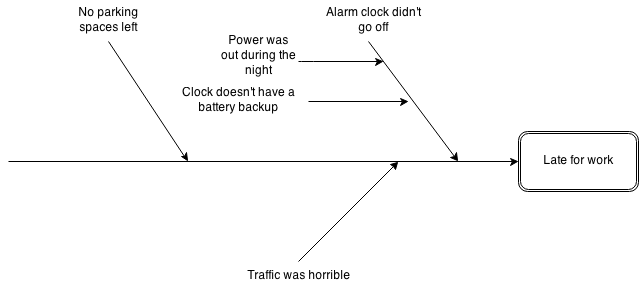
\includegraphics[width=\textwidth]{figures/fishbone-example.png}
	\caption{Fishbone diagram showing the cause analysis of the issue of arriving late for work.}
	\label{figure:fishbone-example}
\end{figure}

\paragraph{Causal Map Analysis}
Bjørnson, Wang and Arisholm~\cite{Wang2012} proposes an alternative to fishbone diagrams in the form of causal map analysis. This is conducted in a similar way to the KJ-sessions, described above. The participants are given post-it notes on which they separately write down the causes of the issue the group is analyzing. They each then present their causes for the rest. When all causes are up on the whiteboard the participants together group the causes were able before they draw cause-effects relationships between the causes indicated by arrows. The group then are allowed to write new notes finding deeper or missing causes and place them in the map. This process continues until the participants are satisfied with the analysis. \autoref{figure:causalmap-example} gives an example of a causal map identifying the causes of the issue of arriving late for work.

\begin{figure}[h!]
	\centering
	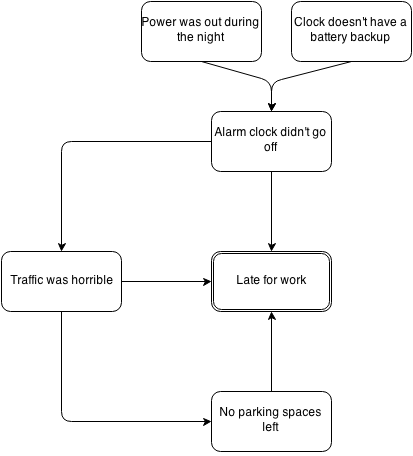
\includegraphics[width=0.7\textwidth]{figures/causalmap-example.png}
	\caption{Causal map showing the cause analysis of the issue of arriving late for work.}
	\label{figure:causalmap-example}
\end{figure}

\subsubsection{Which Technique to Use?}
 
\subsection{After the Retrospective}

\section{Enthusiasm for the Agile Retrospective}

\clearpage

\part{Discussion}
\clearpage

\bibliography{references}
\bibliographystyle{plain}
\end{document}